\documentclass[a4paper]{article}

%opening

\title{\huge Assignment 1: Software Requirements Specification and Technology Neutral Process Design
\\COS 301 Team Alpha Project
\\Version 1.0}

\author{\\\\Amy Lochner 14038600\\ Avinash Singh 14043778 \\
Christiaan Nel 14029368\\ Christiaan Saaiman 12059138 \\
Gerard van Wyk 14101263\\ Marc Antel 12026973\\
Themba Mbhele 14007950
\\
\\
\\\textit{https://github.com/AvinashSingh786/COS301-Alpha.git}
\\
\\
\\ University Of Pretoria\\}

\date{February 2016}

\usepackage{graphicx}
\usepackage{float}

\begin{document}

\maketitle
% No page number to cover pag
\pagenumbering{gobble}
\newpage
% start page numbering


% Generate Table of Contents

\tableofcontents
\newpage

\section{Introduction}


\section{Vision}

\section{Background}
\section{Architecture Requirements}
\subsection{Access Channel Requirements}
\subsection{Quality Requirements}
\begin{itemize}
	\item performance
	\item security
	\item maintainability
	\item scalability
	\item 
	\item flexibility
	\item reliability
	\item 
	\item 
	\item 
	\item 
\end{itemize}

\subsection{Integration Requirements}


\begin{itemize}
	\item 
	\item 
	\item 
	\item 
\end{itemize}

\subsection{Architecture Constraints}

\begin{itemize}
	\item HTML (Hypertext Markup Language)
	\item AJAX (Asynchronous JavaScript and XML)
	\item JavaEE (Java Platform Enterprise Edition)
	\item 
	\item 
	\item 
	\item 
	\item 
	
\end{itemize}

\section{Functional Requirements and Application Design}

\subsection{Use Case Prioritization}

\subsection{Use Case/Services Contracts}

\subsection{Required Functionality}
\subsubsection{User-Research System interaction}
\paragraph{\textbf{Description:} The type of user indicates what privileges that user has in the Research system}
\paragraph{\textbf{Normal-user}}
\begin{description}
  \item[$\bullet$] A normal user login to the system if on the system
    \item[$\bullet$] A normal user may add documents to the system
    \item[$\bullet$] A normal user is as an author to a document that they add
    \item[$\bullet$] A normal user may add authors to a document
    \item[$\bullet$] A normal user may change authors to a document
    \item[$\bullet$] A normal user may add a document to a conference
    \item[$\bullet$] A normal user may only view their documents
\end{description}
\paragraph{\textbf{Head of Department}}
\begin{description}
  \item[$\bullet$] The head of department may log in to the system
    \item[$\bullet$] The head of department may add users to the system
    \item[$\bullet$] The head of department may remove users from the system
    \item[$\bullet$] The head of department may edit user information on the system
    \item[$\bullet$] The head of department may add documents to the system
    \item[$\bullet$] The head of department may be an author to a document
    \item[$\bullet$] The head of department may add authors to a document
    \item[$\bullet$] The head of department may change authors to a document
    \item[$\bullet$] The head of department may add/remove documents to conferences
    \item[$\bullet$] The head of department may view all documents on the system
\end{description}
\paragraph{\textbf{Admin}}
\begin{description}
  \item[$\bullet$] Admin users may log in to the system
    \item[$\bullet$] Admin users may add users to the system
    \item[$\bullet$] Admin users may remove users from the system
    \item[$\bullet$] Admin users may edit user information on the system
    \item[$\bullet$] Admin users may add documents to the system
    \item[$\bullet$] Admin users may not be an author to documents to the system
    \item[$\bullet$] Admin users may add authors to a document
    \item[$\bullet$] Admin users may change authors to a document
    \item[$\bullet$] Admin users may add/remove documents to conferences
    \item[$\bullet$] Admin users may view all documents on the system
\end{description}
\begin{figure}[H]
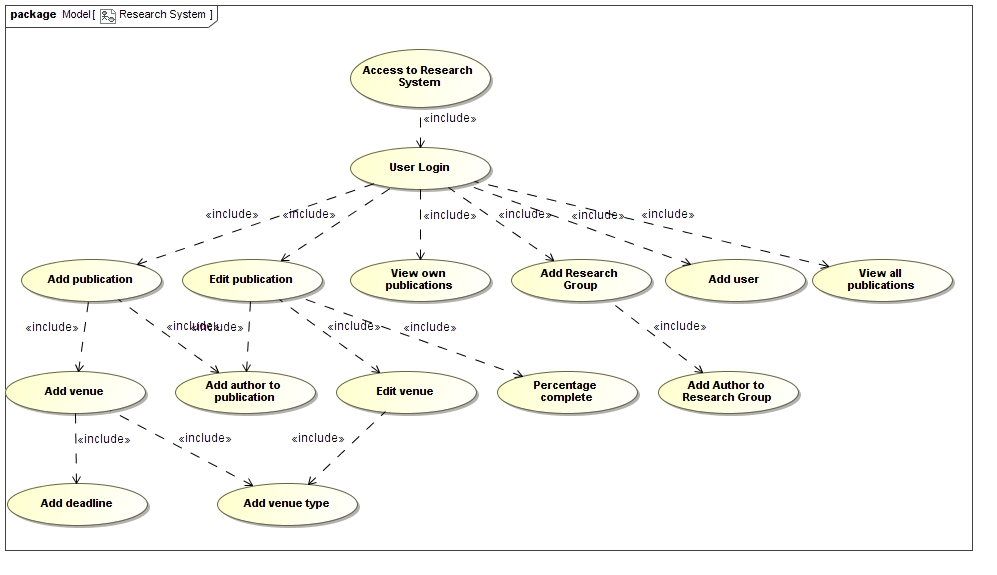
\includegraphics[width=\textwidth]{Overview.jpg}
\caption{Functional Requirements: Overview of Research System \label{overflow}}
\end{figure}
\begin{figure}[H]
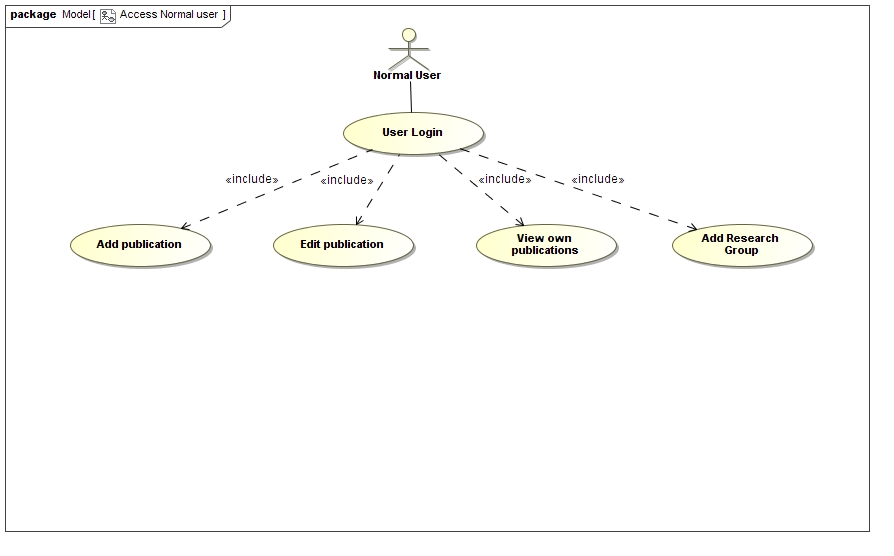
\includegraphics[width=\textwidth]{AccessNormaluser.jpg}
\caption{Functional Requirements: Normal user access privileges \label{overflow}}
\end{figure}
\begin{figure}[H]
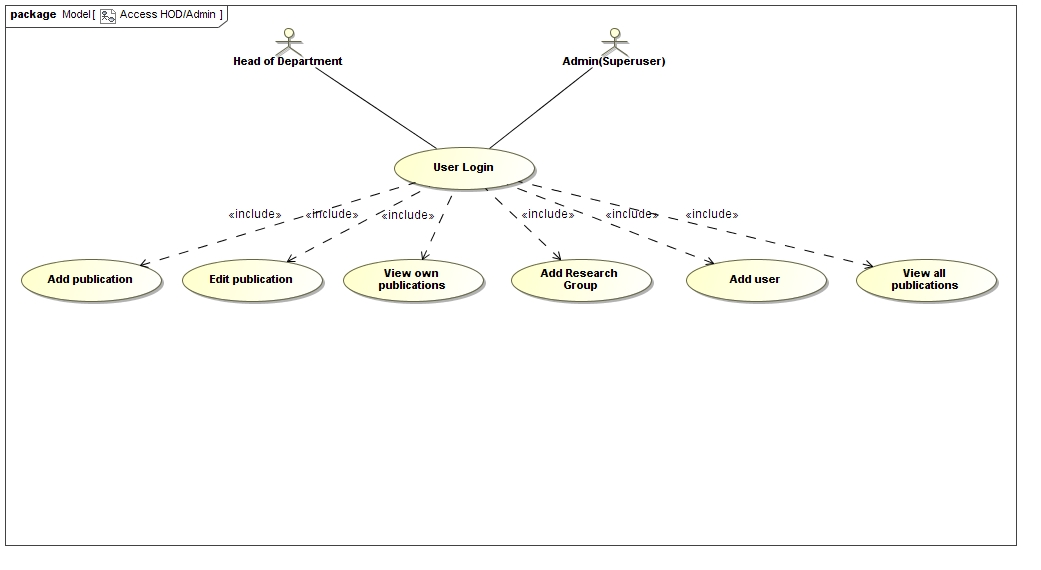
\includegraphics[width=\textwidth]{AccessHODAdmin.jpg}
\caption{Functional Requirements: Superuser(HOD and admin) access privileges \label{overflow}}
\end{figure}
\subsection{Process Specification}
\subsection{Domain Model}


\section{Open Issues}


\end{document}
